% !TEX root = ../Ragni2016.tex

%  ___                 _      _   _
% |   \ ___ ___ __ _ _(_)_ __| |_(_)___ _ _
% | |) / -_|_-</ _| '_| | '_ \  _| / _ \ ' \
% |___/\___/__/\__|_| |_| .__/\__|_\___/_||_|
%                       |_|
\section{Software description}
\label{sec:description}

% Describe the software in as much as is necessary to establish a vocabulary needed to explain
% its impact.

%    _          _    _ _          _
%   /_\  _ _ __| |_ (_) |_ ___ __| |_ _  _ _ _ ___
%  / _ \| '_/ _| ' \| |  _/ -_) _|  _| || | '_/ -_)
% /_/ \_\_| \__|_||_|_|\__\___\__|\__|\_,_|_| \___|
\subsection{Software Architecture}
\label{sec:architecture}

% Give a short overview of the overall software architecture; provide a pictorial component overview
% or similar (if possible). If necessary provide implementation details.

\ragnicas~is an object oriented ASD gem that supports computer algebra routines such as simplifications and substitutions. When gem is required, it overloads methods of \Fixnum~and \Float~classes, making them compatible with fundamental symbolic classes.

Each symbolic expression (or operation) is the instance of an object, that inherits from a common virtual ancestor: \CASOp. An operation encapsulates sub-operations recursively, building a tree, that is the mathematical equivalent of function composition:
\begin{equation}
\left( f \, \circ \, g \right)
\end{equation}

\begin{figure}[ht!]
\centering
%\begin{tikzpicture}[->,>=stealth',shorten >=1pt,auto,node distance=2.5cm]
  \tikzstyle{naryop}=[draw=black]
  \tikzstyle{constant}=[draw=red,text=red]
  \tikzstyle{variables}=[draw=blue,text=blue]
  \tikzstyle{binaryop}=[draw=black,fill=black!20]

  % Nodes
  \node[state]           (Sum)                          {$x_0 + x_1$};

  \node[state]           (Prod)  [below left of=Sum]    {$x_0 \cdot x_1$};
  \node[state,constant]  (Zero)  [below right of=Sum]   {$0$};

  \node[state,constant]  (Two)   [below left of=Prod]   {$2$};
  \node[state,binaryop]  (Pow)   [below right of=Prod]  {$x^y$};

  \node[state,variables] (X)     [below left of=Pow]    {$z$};
  \node[state,binaryop]  (Minus) [below right of=Pow]   {$x - y$};

  \node[state,constant]  (Two2)  [below left of=Minus]  {$2$};
  \node[state,constant]  (One)   [below right of=Minus] {$1$};

  % Legend
  \node[naryop]    (legend-Nary)   [below of=One,yshift=1cm] {\makebox[1.7cm]{\scriptsize\texttt{CAS::NaryOp}}};
  \node[binaryop]  (legend-Binary) [left of=legend-Nary]    {\makebox[1.7cm]{\scriptsize\texttt{CAS::BinaryOp}}};
  \node[variables] (legend-vars)   [below of=legend-Nary,yshift=2cm]     {\makebox[1.7cm]{\scriptsize\texttt{CAS::Variable}}};
  \node[constant]  (legend-const)  [left of=legend-vars]     {\makebox[1.7cm]{\scriptsize\texttt{CAS::Constant}}};
  \node (legendText) [left of=legend-Binary] {\scriptsize Classes:};

  % Origin
  \node (equation) [above of=Sum,xshift=-2.5cm] {$\dfrac{d}{dz}\,\left(z^2 + 1\right) = 2\,z^{(2 - 1)}+0$};

  \path (Sum)      edge node [anchor=south east] {\scriptsize $x_0 \leftarrow 2\,z^{(2 - 1)}$} (Prod)
                   edge node {\scriptsize $x_1 \leftarrow 0$}                                  (Zero)
        (Prod)     edge node [anchor=south east] {\scriptsize $x_0 \leftarrow 2$}              (Two)
                   edge node                     {\scriptsize $x_1 \leftarrow z^{(2-1)}$}      (Pow)
        (Pow)      edge node [anchor=south east] {\scriptsize $x \leftarrow z$}                (X)
                   edge node                     {\scriptsize $y \leftarrow (2 - 1)$}          (Minus)
        (Minus)    edge node [anchor=south east] {\scriptsize $x \leftarrow 2$ }               (Two2)
                   edge node                     {\scriptsize $y \leftarrow 1$ }               (One)
        (equation) edge                                                                        (Sum);
\end{tikzpicture}

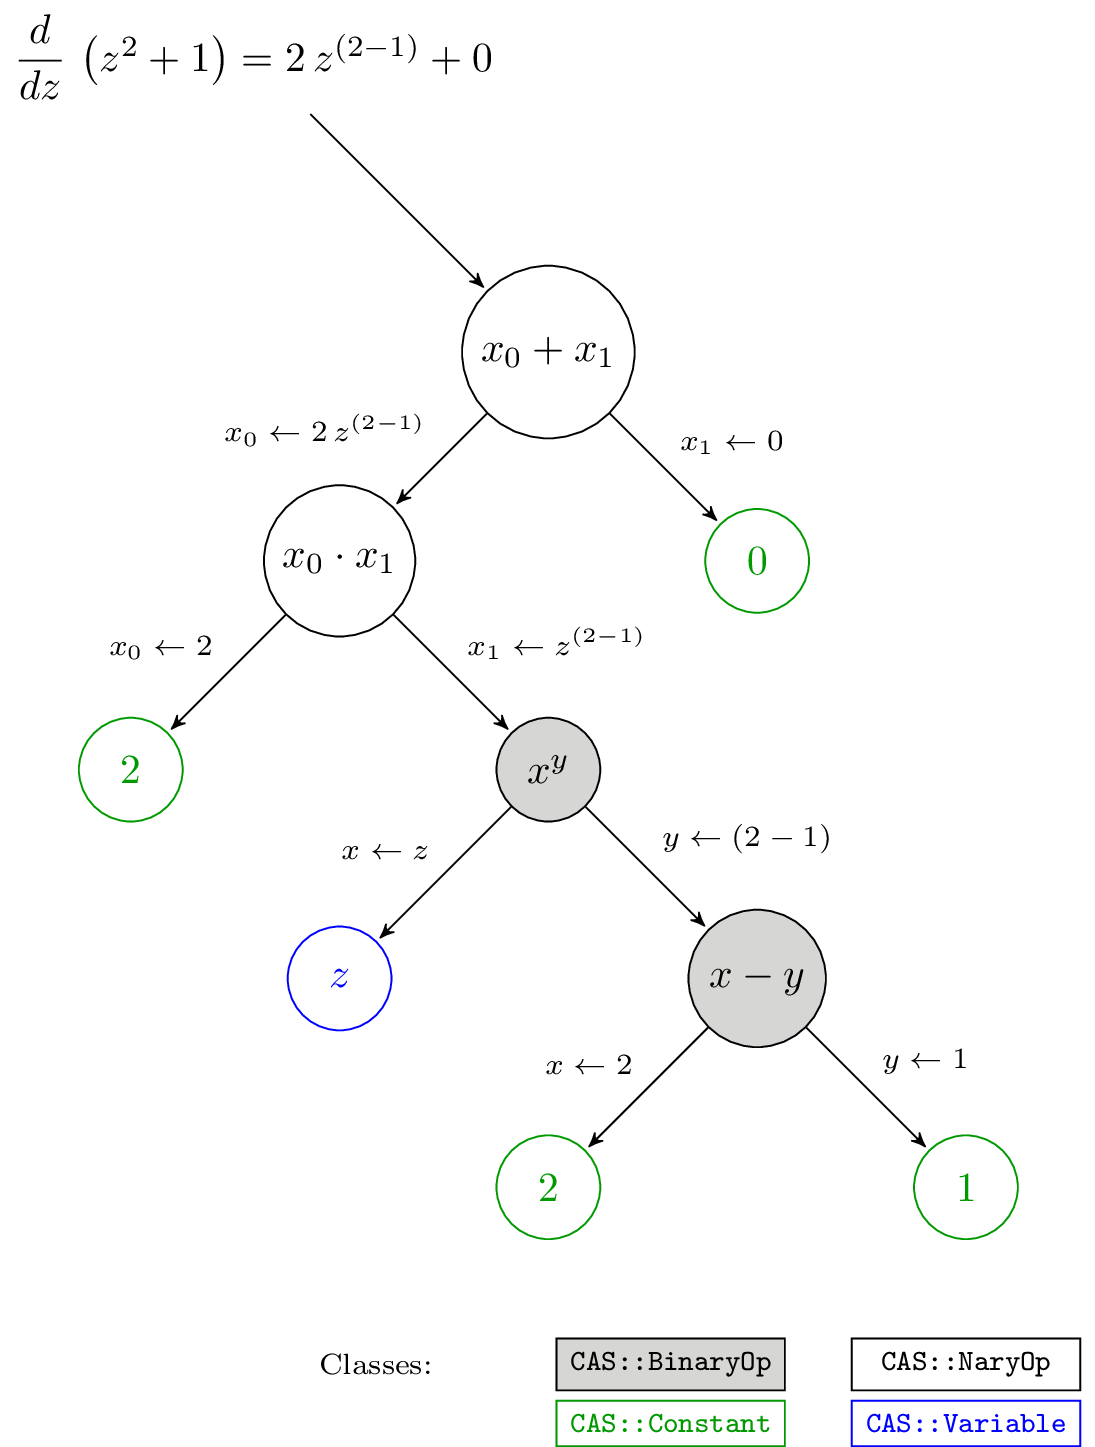
\includegraphics{img/graph-ex.png}
\caption{\label{fig:graph}Tree of the expression derived in Listing~\ref{code:example-diff}}
\end{figure}

When a new operation is created, it is appended to the tree. The number of branches are determined by the parent container class of the current symbolic function. There are three possible containers:
\begin{description}
  \item[\CASOp] single sub-tree operation---e.g.~$\sin(\cdot)$.
  \item[\CASBinaryOp] dual sub-tree operation---e.g.~exponent $x^y$---that inherits from~\CASOp.
  \item[\CASNaryOp] operation with arbitrary number of sub-tree---e.g.~sum $x_1 + \cdots + x_N$---that inherits from~\CASOp.
\end{description}
Fig.~\ref{fig:graph} contains a graphical representation of a expression tree. The different kind of containers allows to introduce some properties---i.e.~\emph{associativity} and \emph{commutativity} for sums and multiplications~\cite{cohen2003computer}. Each container exposes the sub-tree as instance properties. \review{Basic} containers interfaces and inheritances are shown in Fig.~\ref{fig:uml-container}. \review{For a complete overview of all classes and inheritance, please refer to software documentation.}

The terminal leaves of the graph are the classes \CASConstant, \CASVariable~and \CASFunction. The first models a simple numerical value, while the second represents an independent variable, that can be used to perform derivatives and evaluations, and the latter is a prototype of implicit functions. Those leaves exemplify only real scalar expressions, with definition of complex, vectorial, and matricial extensions as milestones for the next major release.

The symbolic differentiation (\CASOpdiff) explores the graph until it reaches ending nodes. A terminal node is the starting point for derivatives accumulation, the mathematical equivalent of the chain rule:
\begin{equation}
\left( f  \, \circ \, g \right)' \: = \:
\left( f' \, \circ \, g \right) \: g'
\end{equation}
The recursiveness is used also for simplifications (\CASOpsimplify), substitutions (\CASOpsubs), evaluations (\CASOpcall) and code generation.

\begin{figure}[ht!]
\centering
%\begin{tikzpicture}
\umlclass[type=abstract]{CAS::Op}{
x : CAS::Op
}{
\umlvirt{ diff(CAS::Op) : CAS::Op } \\
\umlvirt{ subs(Hash) : CAS::Op    } \\
\umlvirt{ call(Hash) : Numeric } \\
\umlvirt{ simplify : CAS::Op      }
}

\umlclass[type=abstract,x=3,y=-5.5]{CAS::BinaryOp}{
x : CAS::Op \\
y : CAS::Op
}{}

\umlclass[type=abstract,x=3,y=-10.5]{CAS::NaryOp}{
x : Array
}{}

\umlemptyclass[x=8]{CAS::Sin}
\umlemptyclass[x=8,y=-2]{CAS::Log}
\umlsimpleclass[x=8,y=-3.5,draw=white]{...}

\umlemptyclass[x=8,y=-5.5]{CAS::Diff}
\umlemptyclass[x=8,y=-7.5]{CAS::Pow}
\umlsimpleclass[x=8,y=-9,draw=white]{...}

\umlemptyclass[x=8,y=-10.5]{CAS::Sum}
\umlemptyclass[x=8,y=-12.5]{CAS::Mul}
\umlsimpleclass[x=8,y=-14,draw=white]{...}


% Inheritance
\umlinherit[geometry=|-,anchor2=east]{CAS::BinaryOp}{CAS::Op}
\umlinherit[geometry=|-,anchor2=east]{CAS::NaryOp}{CAS::Op}

\umlinherit[geometry=--,anchor1=east,anchor2=east]{CAS::Sin}{CAS::Op}
\umlinherit[geometry=-|-,anchor1=east,anchor2=east]{CAS::Log}{CAS::Op}

\umlinherit[geometry=--,anchor1=east,anchor2=east]{CAS::Diff}{CAS::BinaryOp}
\umlinherit[geometry=-|-,anchor1=east,anchor2=east]{CAS::Pow}{CAS::BinaryOp}

\umlinherit[geometry=--,anchor1=east,anchor2=east]{CAS::Sum}{CAS::NaryOp}
\umlinherit[geometry=-|-,anchor1=east,anchor2=east]{CAS::Mul}{CAS::NaryOp}

\end{tikzpicture}

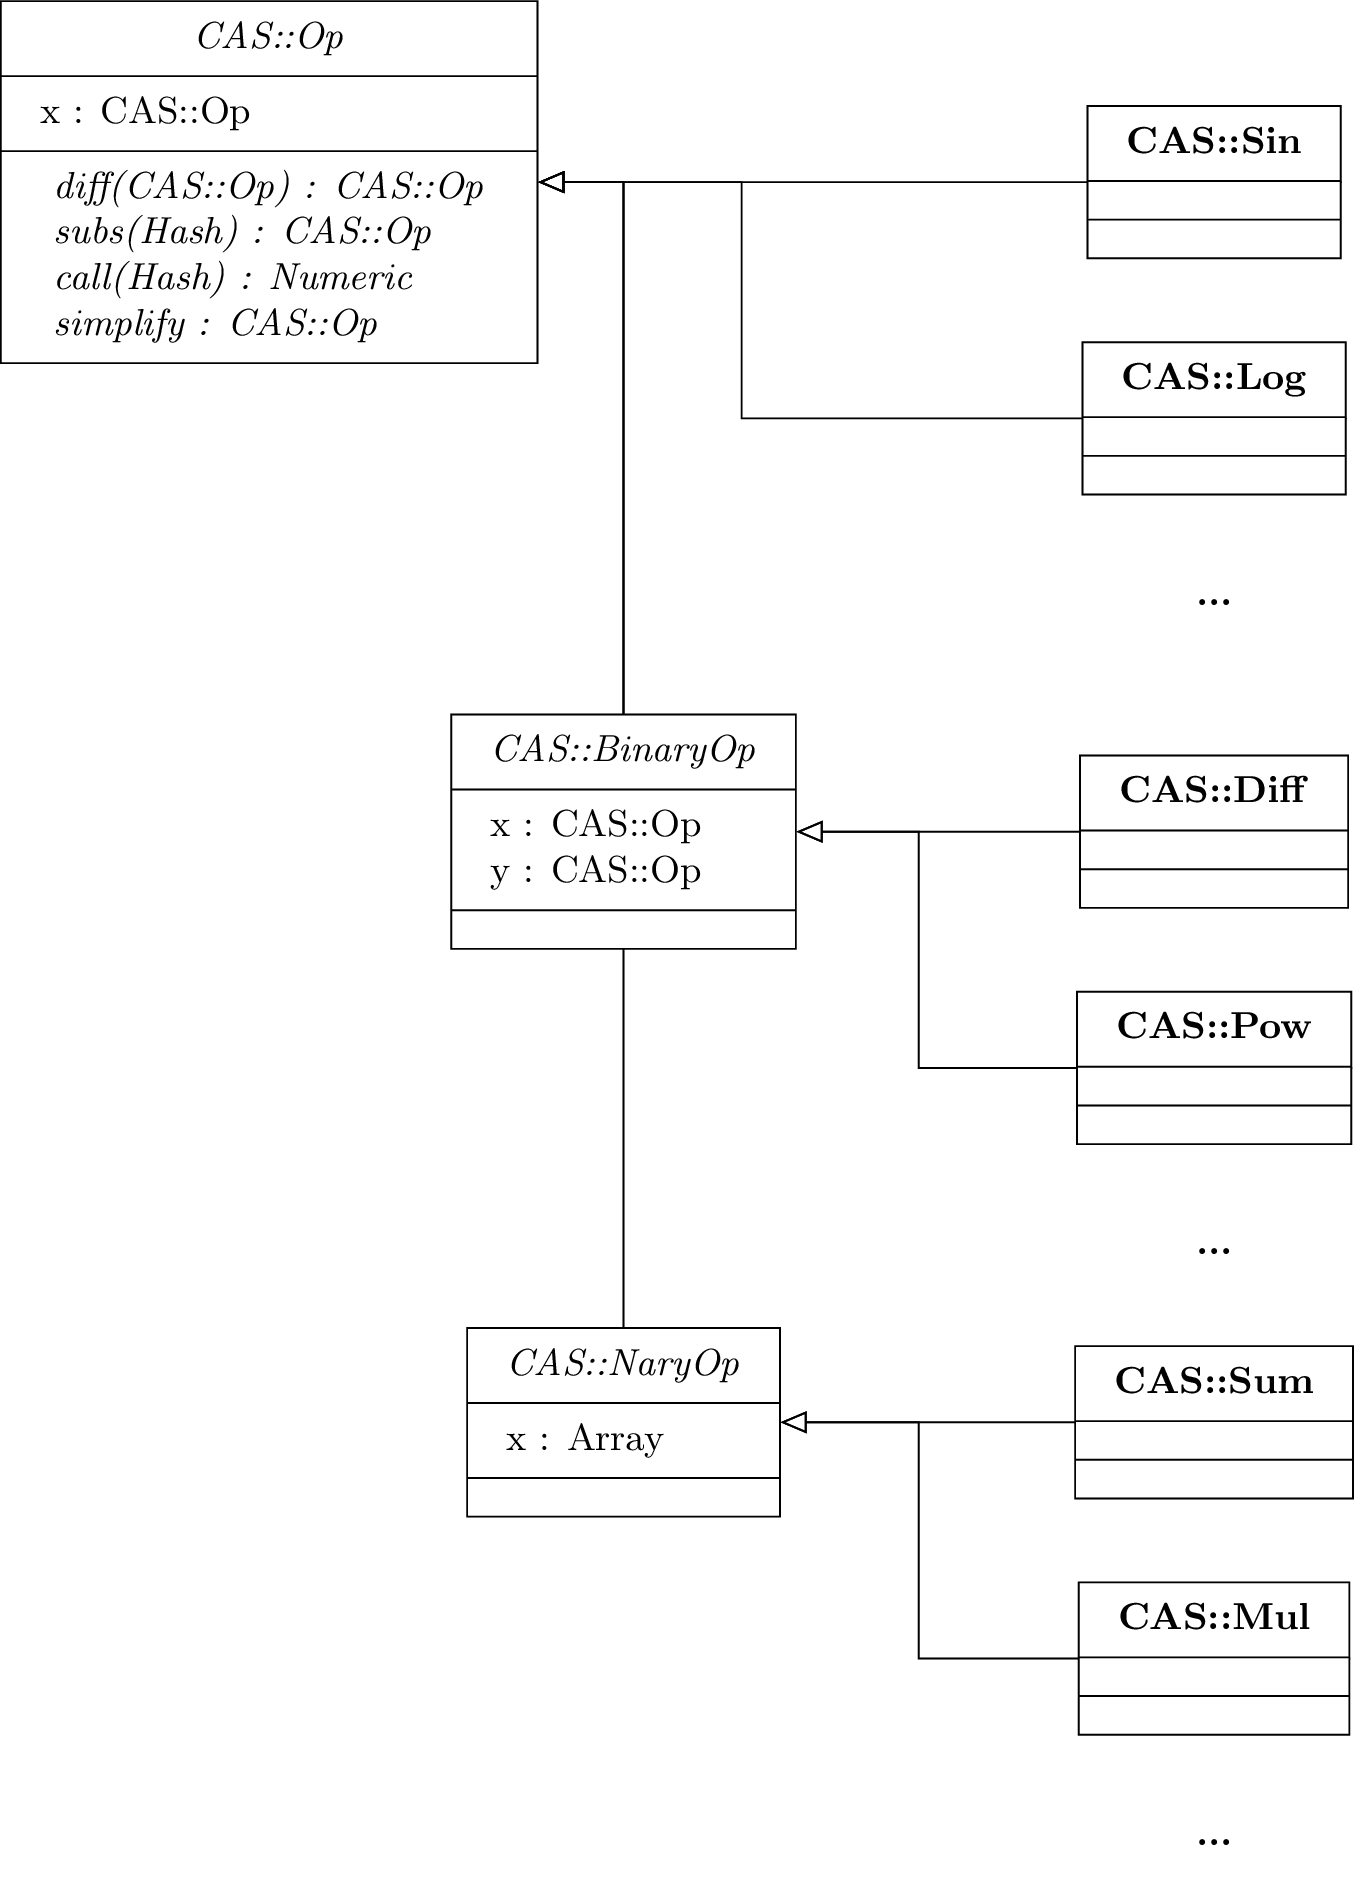
\includegraphics{img/class-struct.png}
\caption{\label{fig:uml-container}Reduced version of classes interface and inheritance. \review{The figure depicts the basic abstract class \CASOp, from which the \emph{single argument} operations inherit. \CASOp~is also the ancestor for other kind of containers, namely the \CASBinaryOp~and \CASNaryOp, the models of container with \emph{two} and \emph{more arguments}}}
\end{figure}

%  ___             _   _               _ _ _   _
% | __|  _ _ _  __| |_(_)___ _ _  __ _| (_) |_(_)___ ___
% | _| || | ' \/ _|  _| / _ \ ' \/ _` | | |  _| / -_|_-<
% |_| \_,_|_||_\__|\__|_\___/_||_\__,_|_|_|\__|_\___/__/
\subsection{Software Functionalities}
\label{sec:functionalities}

%\subsubsection{Software installation and prerequisites}
\subsubsection{Basic Functionalities}

\emph{No additional dependencies are required}. The gem can be installed through the \emph{rubygems.org} provider\footnote{\texttt{gem install Mr.CAS}}. Gem functionalities are required using the Kernel method: \texttt{require 'Mr.CAS'}. All methods and classes are encapsulated in the module \texttt{CAS}.

%\subsubsection{Basic Functionalities}

% Present the major functionalities of the software.
Symbolic Differentiation (SD) is performed with respect to independent variables (\CASVariable) through forward accumulation, even for implicit functions. The differentiation is done by the method \CASOpdiff, having a \CASVariable~as argument, as shown in Listing~\ref{code:example-diff}.

\noindent%
\lstinputlisting[caption={Differentiation example},label={code:example-diff}]{./scripts/listing_01.rb}

Automatic differentiation (AD) is included as a plugin and exploits the properties of dual numbers to efficiently perform differentiation, see~\cite{bartholomew2000automatic} for further details. The AD strategy is useful in case of complex expressions, where explicit derivative's tree may exceed the call stack depth.

Simplifications are not executed automatically, after differentiation. Each node of the tree knows rules for simplify itself, and rules are called recursively, exactly like ASD.\@ Simplifications that require a \emph{heuristic expansion} of the sub-graph---i.e.\ some trigonometric identities---are not defined for now, but can be easily achieved through substitutions, as shown in Listing~\ref{code:example-simp}.

\noindent%
\lstinputlisting[caption={Simplification example},label={code:example-simp}]{./scripts/listing_02.rb}

The tree is numerically evaluated when the independent variables values are provided in a feed dictionary. The graph is reduced recursively to a single numeric value, as shown in Listing~\ref{code:example-call}.

\noindent%
\lstinputlisting[caption={Tree evaluation example},label={code:example-call}]{./scripts/listing_03.rb}


Symbolic expressions can be used to create comparative expressions, that are stored in special container classes, modeled by the ancestor \CASExpression---for example, $f(\cdot) \geq g(\cdot)$. This allow the definition of piecewise functions, \review{in \CASPiecewise. Internally, $\max(\cdot)$ and $\min(\cdot)$ functions are declared as operations that inherits from \CASPiecewise}---for example, $\max(f(\cdot), g(\cdot))$. Usage is shown in Listing~\ref{code:example-expr}.

\noindent%
\lstinputlisting[caption={Expressions and Piecewise functions},label={code:example-expr}]{./scripts/listing_04.rb}

\subsubsection{Meta-programming and Code-Generation}

\ragnicas~is developed explicitly for {meta\-programming} and code generation. Expressions can be exported as source code or used as prototypes for callable \emph{closures} (the \texttt{Proc} object in Listing~\ref{code:example-proc}):

\noindent%
\lstinputlisting[caption={Graph evaluation example},label={code:example-proc}]{./scripts/listing_05.rb}

Compiling a closure of a tree is like making its snapshot, thus any further manipulation of the expression does not update the callable object. This drawback is balanced by the faster execution time of a \texttt{Proc}: when a graph needs \emph{only to be evaluated}, transforming it in a \emph{closure} reduces the execution time---for example, in a iterative algorithm, where a closure is called at each iteration.

Code generation should be flexible enough to export expression trees in a user's target language. Generation methods for common languages are included in specific \emph{plugins}. Users can furthermore expand exporting capabilities by writing specific exportation rules, overriding method for existing plugin, or designing their own exporter, like the one shown in Listing~\ref{code:example-exporting}:

\noindent%
\lstinputlisting[caption={Example of Ruby code generation plugin},label={code:example-exporting}]{./scripts/listing_06.rb}
